\section{Risposte alle domande}

\subsection{Domanda 1}

\textit{Eseguite i tre algoritmi che avete implementato (Prim, Kruskal naive e
Kruskal efficiente) sui grafi del dataset. Misurate i tempi di calcolo dei tre algoritmi e
create un grafico che mostri la variazione dei tempi di calcolo al variare del numero di
vertici nel grafo. Confrontate i tempi misurati con la complessità asintotica attesa dalla
teoria. Per ognuna delle istanze del problema, riportate il peso del minimum spanning tree
ottenuto dagli algoritmi.}

Abbiamo implementato il codice in Python per l'esecuzione dei tre algoritmi su tutto il dataset fornito. I risultati, che sono stati riportati in modo dettagliato e con i relativi pesi anche nella sezione appendice, sono riportati di seguito.

\subsubsection{Risultati con Kruskal naive}


\begin{figure}[H]
	\centering
	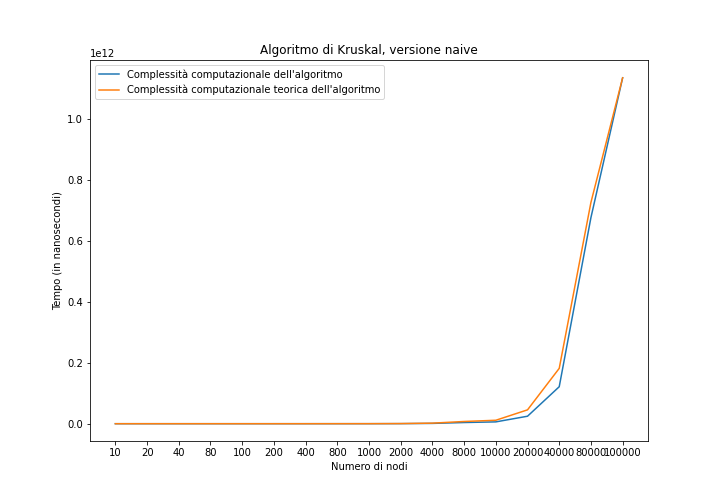
\includegraphics[width=0.9\textwidth]{res/images/graph-no-rep/kruskal_naive_senza_ripetizioni.png}
    \caption{Complessità di Kruskal Naive con una esecuzione per ogni quartetto di grafi con uguale numero di nodi.}
	\label{fig:kruskalnr}
\end{figure}

\begin{figure}[H]
	\centering
	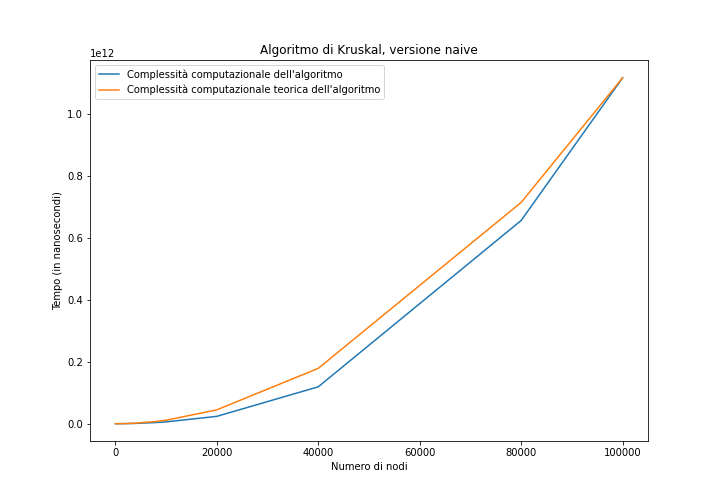
\includegraphics[width=1\textwidth]{res/images/graph-complexity/kruskal_naive.png}
    \caption{Complessità di Kruskal Naive con \(k\) esecuzioni ripetute per ogni quartetto di grafi con uguale numero di nodi.}
	\label{fig:kruskal}
\end{figure}

Nel grafico appena illustrato (fig. \ref{fig:kruskal}) è riportata la complessità computazionale attesa (in giallo) ed effettiva (in blu) per l'algoritmo di Kruskal Naive con più esecuzioni dell'algoritmo. 
Come si può evincere dall'immagine, la curva della complessità effettiva rimane leggermente al di sotto della curva teorica, e pertanto le due complessità sono equiparabili. % mustaches


\subsubsection{Risultati con Kruskal Union Find}

\begin{figure}[H]
	\centering
	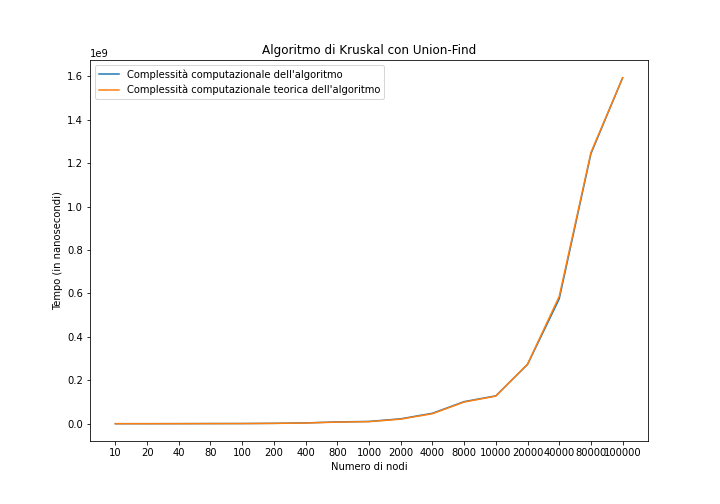
\includegraphics[width=0.70\textwidth]{res/images/graph-no-rep/kruskal_uf_senza_ripetizioni.png}
    \caption{Complessità di Kruskal Union Find con una esecuzione per ogni quartetto di grafi con uguale numero di nodi.}
	\label{fig:kruskal_ufnr}
\end{figure}

\begin{figure}[H]
	\centering
	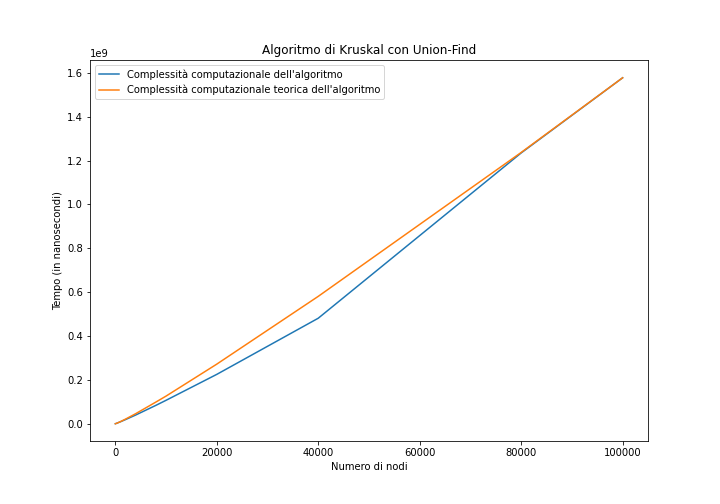
\includegraphics[width=0.70\textwidth]{res/images/graph-complexity/kruskal_union_find.png}
	\caption{Complessità di Kruskal Union Find con \(k\) esecuzioni ripetute per ogni quartetto di grafi con uguale numero di nodi.}
	\label{fig:kruskal_uf}
\end{figure}

\begin{figure}[H]
	\centering
	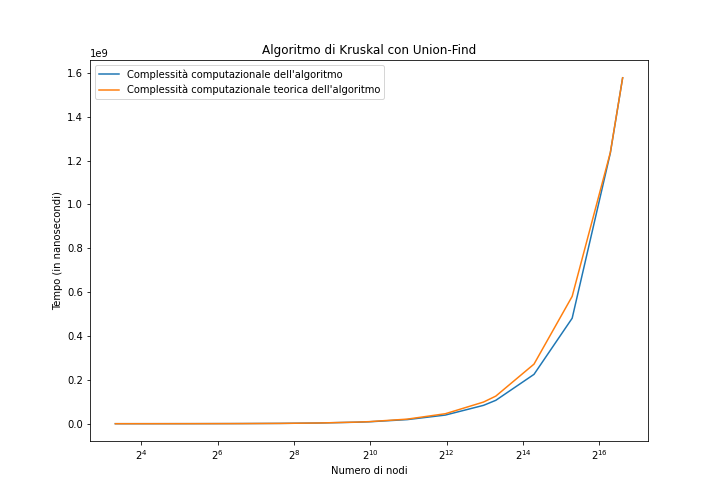
\includegraphics[width=1\textwidth]{res/images/graph-log/kruskal_union_find_scala_logaritmica.png}
	\caption{Complessità di Kruskal Union Find con \(k\) esecuzioni ripetute per ogni quartetto di grafi con uguale numero di nodi, in scala logaritmica.}
	\label{fig:kruskal_log}
\end{figure}

Nei grafici appena illustrati (fig. \ref{fig:kruskal_uf}, \ref{fig:kruskal_log}) è riportata la complessità computazionale attesa (in giallo) ed effettiva (in blu) per l'algoritmo di Kruskal Union Find; il grafico \ref{fig:kruskal_log} è riportato in scala logaritmica per meglio apprezzare l'andamento asintotico dell'algoritmo.
Come si può evincere dall'immagine, anche in questo caso la curva della complessità effettiva rimane leggermente al di sotto della curva teorica.


\subsubsection{Risultati con Prim}

\begin{figure}[H]
	\centering
	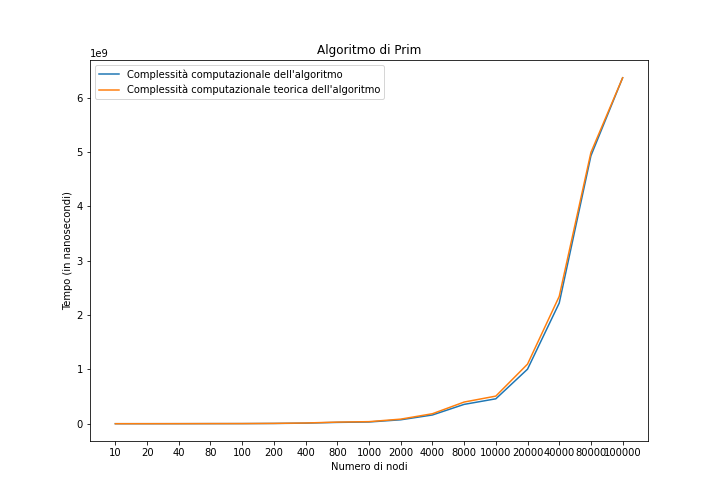
\includegraphics[width=0.7\textwidth]{res/images/graph-no-rep/prim_senza_ripetizioni.png}
    \caption{Complessità di Prim con una esecuzione per ogni quartetto di grafi con uguale numero di nodi.}
	\label{fig:primnr}
\end{figure}

\begin{figure}[H]
	\centering
	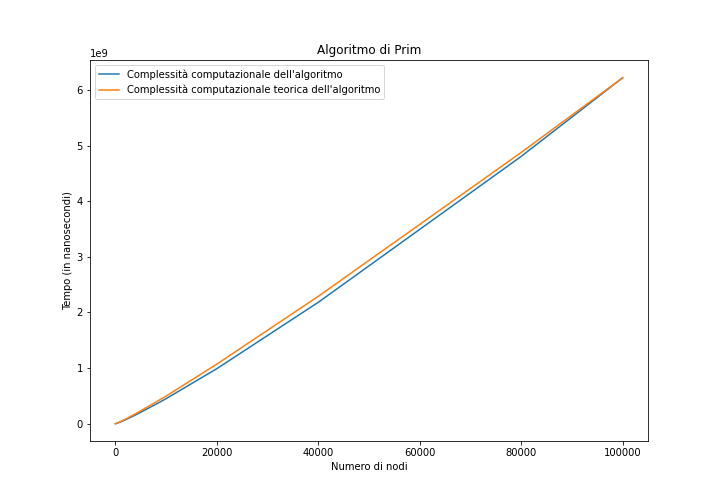
\includegraphics[width=0.7\textwidth]{res/images/graph-complexity/prim.png}
		\caption{Complessità di Prim con \(k\) esecuzioni ripetute per ogni quartetto di grafi con uguale numero di nodi.}
	\label{fig:prim}
\end{figure}

\begin{figure}[H]
	\centering
	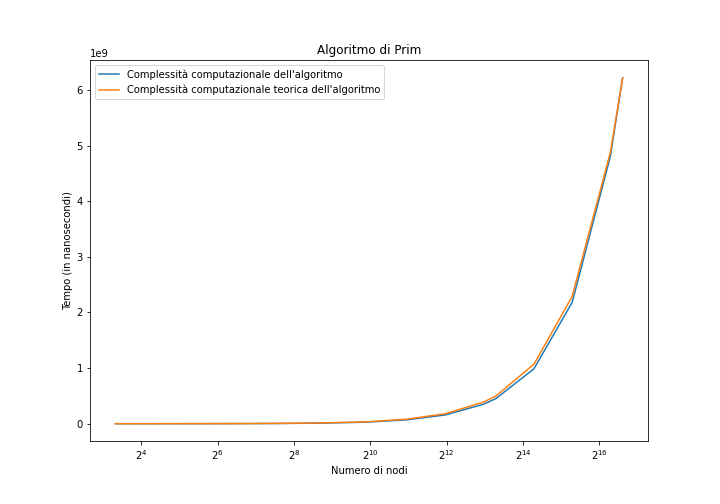
\includegraphics[width=1\textwidth]{res/images/graph-log/prim_scala_logaritmica.png}
	\caption{Complessità di Prim con \(k\) esecuzioni ripetute per ogni quartetto di grafi con uguale numero di nodi, in scala logaritmica.}
	\label{fig:prim_log}
\end{figure}


Nei grafici appena illustrati (fig. \ref{fig:prim}, \ref{fig:prim_log}) è riportata la complessità computazionale attesa (in giallo) ed effettiva (in blu) per l'algoritmo di Prim; il grafico \ref{fig:prim_log} è riportato in scala logaritmica per meglio apprezzare l'andamento asintotico dell'algoritmo.
Come si può evincere dall'immagine, anche in questo caso la curva della complessità effettiva rimane leggermente al di sotto della curva teorica.


% ==================================================================================================


\subsection{Domanda 2}
\textit{Commentate i risultati che avete ottenuto: come si comportano gli
algoritmi rispetti alle varie istanze? C'è un algoritmo che riesce sempre a fare meglio
degli altri? Quale dei tre algoritmi che avete implementato è più efficiente?}


Analizzando i tre algoritmi abbiamo appurato che nel caso di Kruskal Naive l'algoritmo richiede un tempo medio di esecuzione in un ordine decisamente superiore rispetto a Kruskal UF e Prim. Infatti, il tempo medio calcolato nel caso del quartetto contenente il maggior numero di nodi (100000) i risultati sono stati i seguenti:

\begin{table}[H]\centering
	\begin{tabular}{l|l|l|l|l}
        \textbf{Num. di nodi} & \textbf{Datasets} & \textbf{Kruskal naive [s]} & \textbf{Kruskal UF [s]} & \textbf{Prim [s]} \\
    \hline
	100000 & 65, 66, 67, 68 & 1117.8413379  & 1.5777018  & 6.2187226 
	\end{tabular}
\end{table}

Confrontando invece i risultati dei grafi con un minor numero di vertici abbiamo potuto constatare quanto segue:

\begin{table}[H]\centering
	\begin{tabular}{l|l|l|l|l}
        \textbf{Num. di nodi} & \textbf{Datasets} & \textbf{Kruskal naive [s]} & \textbf{Kruskal UF [s]} & \textbf{Prim [s]} \\
    \hline
	10 & 1, 2, 3, 4  & 0.0000450 & 0.0000465 & 0.0000868 \\
    20 & 5, 6, 7, 8  & 0.0001154 & 0.0001138  & 0.0002398 \\
    40 & 9, 10, 11, 12  & 0.0002559 & 0.0002456  & 0.0005888 \\
	\end{tabular}
\end{table}

\noindent I tempi rilevati con Kruskal Naive risultano più vicini agli altri algoritmi dal momento che avvicinandoci a un minor numero di nodi non si può apprezzare una differenza di tempi di esecuzione media, visto che per valori di \(n\) che tendono a 0 le funzioni delle complessità computazionali degli algoritmi restituiscono dei valori molto simili. 

\subsubsection{Confronto Prim-Kruskal Union Find}


\begin{figure}[H]
	\centering
	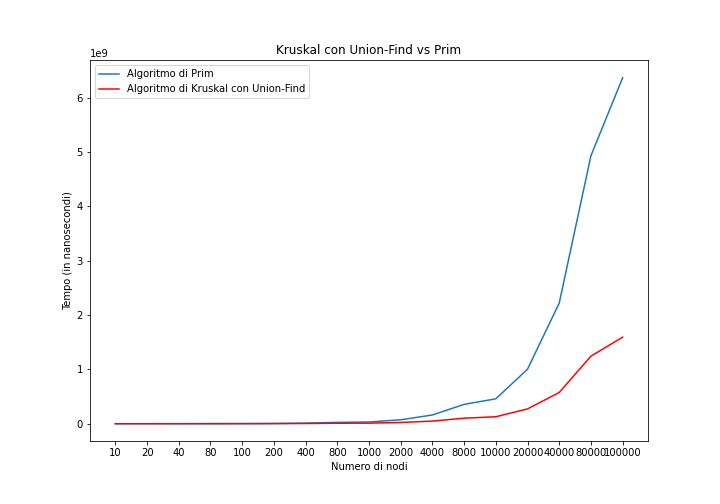
\includegraphics[width=0.7\textwidth]{res/images/graph-no-rep/kruskal_uf_vs_prim_senza_ripetizioni.png}
    \caption{Confronto tra Prim e Kruskal UF con una esecuzione per ogni quartetto di grafi con uguale numero di nodi.}
	\label{fig:krukal_vs_primnr}
\end{figure}


\begin{figure}[H]
	\centering
	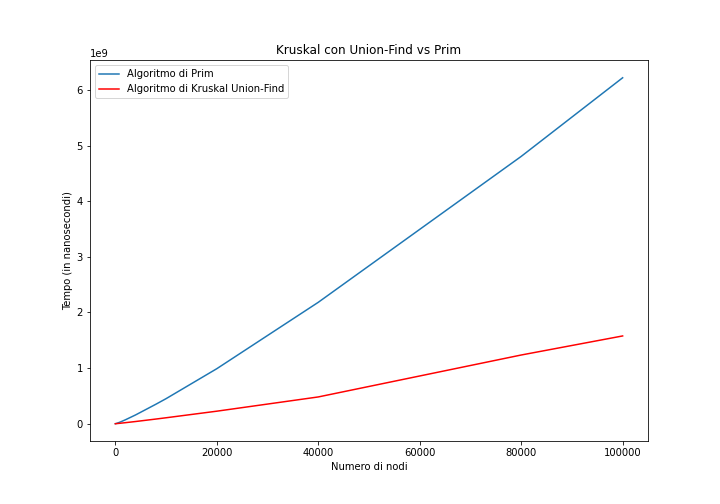
\includegraphics[width=0.75\textwidth]{res/images/graph-complexity/kruskal_uf_vs_prim.png}
	\caption{Confronto tra Prim e Kruskal UF con \(k\) esecuzioni ripetute per ogni quartetto di grafi con uguale numero di nodi.}
    \label{fig:krukal_vs_prim}
\end{figure}

\begin{figure}[H]
	\centering
	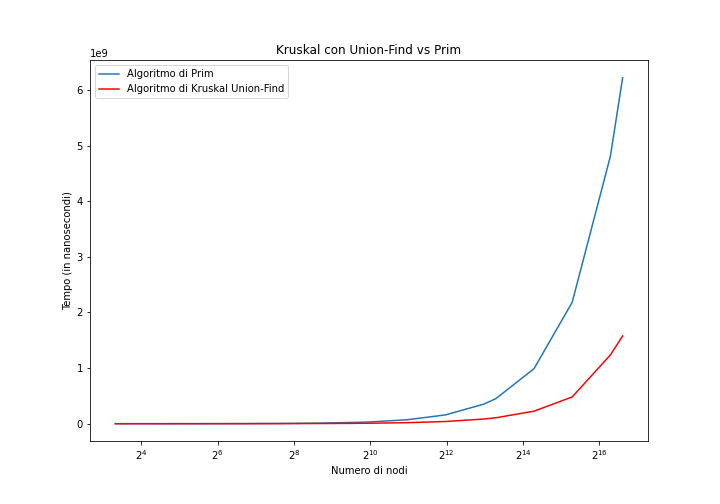
\includegraphics[width=0.75\textwidth]{res/images/graph-log/kruskal_uf_vs_prim_scala_logaritmica.png}
	\caption{Confronto tra Prim e Kruskal UF con \(k\) esecuzioni ripetute per ogni quartetto di grafi con uguale numero di nodi, in scala logaritmica.}
	\label{fig:kruskal_vs_primlog}
\end{figure}


Nei grafici appena illustrati (fig. \ref{fig:krukal_vs_primnr}, \ref{fig:krukal_vs_prim}, \ref{fig:kruskal_vs_primlog}) sono riportati tre confronti tra l'algoritmo di Kruskal Union Find e l'algoritmo di Prim: i primi due in scala lineare e il terzo in scala logaritmica. In tutti e tre i casi è possibile vedere chiaramente che \textbf{l'algoritmo di Kruskal UF risulta essere più efficiente rispetto all'algoritmo di Prim}, dal momento che il tempo di esecuzione medio su un quartetto di grafi è moderatamente più basso per Kruskal UF. Da questo pertanto possiamo concludere che l'algoritmo di Kruskal UF tende a fare sempre meglio rispetto agli altri.
